\documentclass{article}

\usepackage{amsmath,amssymb,amsthm,graphicx,setspace}
\usepackage[margin=1in]{geometry}
\usepackage[longnamesfirst]{natbib}
\bibliographystyle{ecta}
\newtheorem{theorem}{Theorem}
\onehalfspacing
\usepackage{enumerate}
\usepackage[table]{xcolor}
\usepackage{titlesec}
\usepackage{booktabs}
\usepackage{placeins} % for fixing table positions using \FloatBarrier

\setlength\parindent{0pt}

\title{AAA \\ \normalsize BBB}
\date{\today}
\author{Your Name \\Email Adress}

\begin{document}

\maketitle

\begin{enumerate}[I]

%--- I ---%
\item \textbf{Single-Variable Linear Probability Model and Probit Models}

% including and referring to an equation
This refers to equation \ref{eq:struct}:

\begin{equation}\label{eq:struct}
    \beta_y y_t' + \gamma_z z_t' = \zeta_t
\end{equation}

% including table 
%\input{graphs/NullRejection}
%\FloatBarrier

% example: including a figure
\begin{figure}
    \centering
    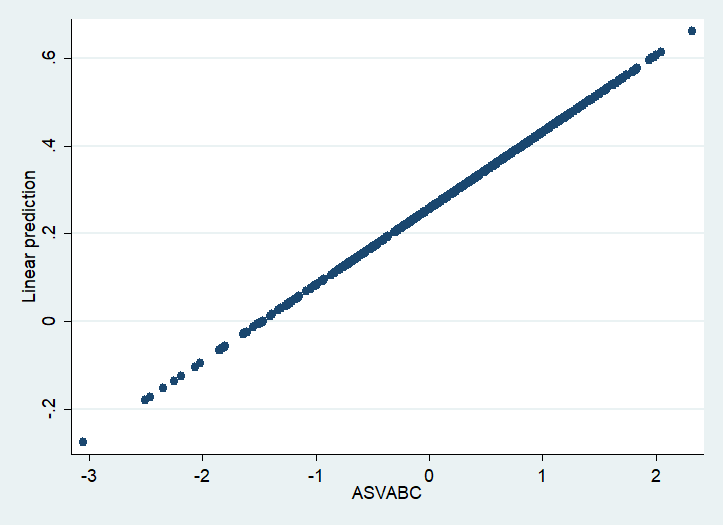
\includegraphics[scale = 0.15]{graphs/linear.png}
    \label{XXX}\caption{XXX}
\end{figure}
\FloatBarrier

\begin{enumerate}[1.]
    \item Answer to I.1
    
    \item \dots
    
    \item Answer to I.9
\end{enumerate}

%--- II ---%
\item\textbf{Multiple-Variable Logit Model}

\dots

%--- III ---%
\item\textbf{Estimating the Human Capital}

\dots

%--- IV ---%
\item\textbf{MLE}

\dots

\end{enumerate}

Table 4.1 Replications 
\begin{table}[htbp]\centering
\caption{Sharp RD estimates of MLDA effects on mortality (Replication of Table 4.1 of AP2014) \label{tab::41}}
\begin{tabular*}{\hsize}{@{\hskip\tabcolsep\extracolsep\fill}l*{8}{c}}
\hline\hline
                    &           1&          se&           2&          se&           3&          se&           4&          se\\
\hline
All                 &        7.66&        1.51&        0.00&        0.00&        9.75&        2.06&        0.00&        0.00\\
MVA                 &        4.53&        0.72&        0.00&        0.00&        4.76&        1.08&        0.00&        0.00\\
Suicide             &        1.79&        0.50&        0.00&        0.00&        1.72&        0.73&        0.00&        0.00\\
Homicide            &        0.10&        0.45&        0.00&        0.00&        0.16&        0.59&        0.00&        0.00\\
External Other      &        0.44&        0.29&        0.00&        0.00&        0.83&        0.37&        0.00&        0.00\\
Internal            &        0.39&        0.54&        0.00&        0.00&        1.69&        0.74&        0.00&        0.00\\
Alcohol             &        0.44&        0.21&        0.00&        0.00&        0.74&        0.33&        0.00&        0.00\\
Sample\_Size         &       48.00&           .&        0.00&        0.00&       24.00&           .&        0.00&        0.00\\
\hline\hline
\multicolumn{9}{l}{\footnotesize Samples in columns 1 and 2 regressions have between 19 and 22 years.}\\
\multicolumn{9}{l}{\footnotesize samples in coulmns 3 and 4 have between 20 and 21 years old.}\\
\multicolumn{9}{l}{\footnotesize Columns 1 and 3 report the results of regressing dependent variable on age.}\\
\multicolumn{9}{l}{\footnotesize columns 2 and 4 report results of regressing dependent variable on age, age-squared}\\
\multicolumn{9}{l}{\footnotesize with their interactions with the over-21 dummy.}\\
\end{tabular*}
\end{table}


\end{document}

